\documentclass[11pt,a4paper]{article}

% =========================================================
% LANGUAGE / ENCODING / TYPOGRAPHY
% =========================================================
\usepackage[T1]{fontenc}
\usepackage[utf8]{inputenc}
\usepackage[brazilian]{babel}
\usepackage{lmodern}
\usepackage{microtype}

% =========================================================
% PAGE
% =========================================================
\usepackage[
    top=2.3cm,
    bottom=2.3cm,
    left=2.5cm,
    right=2.5cm
]{geometry}

\setlength{\parindent}{0pt}
\setlength{\parskip}{0.65em}

% =========================================================
% MATH
% =========================================================
\usepackage{amsmath}
\usepackage{amssymb}
\usepackage{amsthm}
\usepackage{bm}

% =========================================================
% TABLES / FIGURES
% =========================================================
\usepackage{booktabs}
\usepackage{tabularx}
\usepackage{array}
\usepackage{graphicx}
\usepackage{float}

% =========================================================
% VISUAL
% =========================================================
\usepackage{xcolor}
\usepackage[most]{tcolorbox}
\usepackage{titlesec}
\usepackage{enumitem}
\usepackage{fancyhdr}

% =========================================================
% COLORS
% =========================================================
\definecolor{mainblue}{HTML}{243B53}
\definecolor{softblue}{HTML}{EAF0F6}
\definecolor{softgray}{HTML}{F5F6F7}
\definecolor{darkgray}{HTML}{444444}
\definecolor{greenbox}{HTML}{EAF4EE}
\definecolor{orangebox}{HTML}{FFF4E5}

% =========================================================
% LINKS
% =========================================================
\usepackage[
    colorlinks=true,
    linkcolor=mainblue,
    citecolor=mainblue,
    urlcolor=mainblue
]{hyperref}

% =========================================================
% HEADINGS
% =========================================================
\titleformat{\section}
  {\Large\bfseries\color{mainblue}}
  {\thesection.}
  {0.5em}
  {}

\titleformat{\subsection}
  {\large\bfseries\color{darkgray}}
  {\thesubsection}
  {0.5em}
  {}

\titlespacing*{\section}
  {0pt}{1.8em}{0.7em}

\titlespacing*{\subsection}
  {0pt}{1.3em}{0.5em}

% =========================================================
% HEADER / FOOTER
% =========================================================
\pagestyle{fancy}
\fancyhf{}
\fancyhead[L]{\small Projeto QFI}
\fancyhead[R]{\small Informação Funcional para MIS}
\fancyfoot[C]{\thepage}

\renewcommand{\headrulewidth}{0.3pt}

% =========================================================
% CUSTOM BOXES
% =========================================================
\newtcolorbox{mainidea}{
    colback=softblue,
    colframe=mainblue,
    boxrule=0.8pt,
    arc=2mm,
    left=4mm,
    right=4mm,
    top=3mm,
    bottom=3mm
}

\newtcolorbox{definitionbox}[1][]{
    colback=softgray,
    colframe=darkgray,
    boxrule=0.6pt,
    arc=2mm,
    left=4mm,
    right=4mm,
    top=3mm,
    bottom=3mm,
    title=#1,
    fonttitle=\bfseries
}

\newtcolorbox{proposedbox}[1][]{
    colback=greenbox,
    colframe=mainblue,
    boxrule=0.8pt,
    arc=2mm,
    left=4mm,
    right=4mm,
    top=3mm,
    bottom=3mm,
    title=#1,
    fonttitle=\bfseries
}

\newtcolorbox{warningbox}[1][]{
    colback=orangebox,
    colframe=darkgray,
    boxrule=0.6pt,
    arc=2mm,
    left=4mm,
    right=4mm,
    top=3mm,
    bottom=3mm,
    title=#1,
    fonttitle=\bfseries
}

% =========================================================
% TITLE
% =========================================================
\title{
    \vspace{-1cm}
    \textbf{\color{mainblue}
    Informação Funcional Quântica\\[0.2cm]
    no Espaço do Problema}
    \\[0.4cm]
    \large
    Reformulação para Otimização Combinatória\\
    via Maximum Independent Set
}

\author{
    Projeto QFI\\
    \small Rafaella Somoza
}

\date{}

% =========================================================
% DOCUMENT
% =========================================================
\begin{document}

\maketitle

% =========================================================
% OPENING
% =========================================================
\begin{mainidea}

\textbf{Mudança conceitual principal}

Nas versões anteriores deste documento, a distribuição de probabilidade
utilizada na informação funcional era obtida principalmente a partir
do próprio circuito, por exemplo por meio da distribuição de fidelidades.

Nesta reformulação, separamos explicitamente duas ideias:

\begin{center}
\textbf{Funcionalidade}
\quad $\longrightarrow$ \quad
\textbf{espaço do problema}
\end{center}

\begin{center}
\textbf{Circuito quântico}
\quad $\longrightarrow$ \quad
\textbf{mecanismo que redistribui probabilidade}
\end{center}

\textbf{Ideia central:}
a informação funcional pertence à paisagem do problema;
o circuito determina o quanto regiões funcionais dessa paisagem
são acessadas, amplificadas ou concentradas.

\end{mainidea}

\tableofcontents

\newpage

% =========================================================
\section{Hierarquia conceitual da reformulação}
% =========================================================

\begin{center}

\begin{tcolorbox}[
    width=0.90\textwidth,
    colback=softgray,
    colframe=mainblue,
    boxrule=0.6pt,
    arc=2mm
]

\centering

\textbf{Problema $G$}

\vspace{0.15cm}
$\downarrow$

\textbf{Espaço de soluções $\Omega$}

\vspace{0.15cm}
$\downarrow$

\textbf{Hamiltoniano $H(x)$}

\vspace{0.15cm}
$\downarrow$

\textbf{Paisagem funcional}

\vspace{0.15cm}
$\downarrow$

\textbf{Informação funcional intrínseca $I_F(x)$}

\vspace{0.15cm}
$\downarrow$

\textbf{Distribuição do circuito $p_d(x)$}

\vspace{0.15cm}
$\downarrow$

\textbf{Informação funcional intermediária $\langle I_F\rangle_d$}

\vspace{0.15cm}
$\downarrow$

\textbf{Amplificação / ganho funcional}

\vspace{0.15cm}
$\downarrow$

\textbf{Comparação entre profundidades}

\end{tcolorbox}

\end{center}

\begin{mainidea}
\centering
\textbf{
A informação funcional pertence à paisagem do problema;
o circuito quântico determina o quão fortemente essa informação
é acessada, amplificada ou concentrada ao longo da evolução.
}
\end{mainidea}

% =========================================================
\section{Reformulação em torno do Maximum Independent Set}
% =========================================================

\subsection{Espaço do problema}

Seja

\[
G=(V,E)
\]

um grafo com

\[
n=|V|
\]

vértices.

Cada bitstring da base computacional

\[
x=(x_1,\ldots,x_n)\in\{0,1\}^n
\]

representa um subconjunto candidato de vértices.

O espaço completo do problema é:

\begin{definitionbox}[Espaço de soluções]

\[
\boxed{
\Omega=\{0,1\}^n
}
\]

e portanto

\[
\boxed{
|\Omega|=2^n
}
\]

\end{definitionbox}

% ---------------------------------------------------------
\subsection{O Hamiltoniano como paisagem funcional}
% ---------------------------------------------------------

Em vez de utilizar apenas uma função de qualidade abstrata,
usamos o Hamiltoniano do MIS como paisagem funcional primária:

\begin{definitionbox}[Hamiltoniano do MIS]

\[
\boxed{
H(x)
=
A\sum_{(i,j)\in E}x_i x_j
-
B\sum_i x_i
}
\]

\end{definitionbox}

O primeiro termo penaliza a seleção simultânea de vértices adjacentes.

O segundo termo recompensa subconjuntos maiores.

Assim:

\begin{itemize}[leftmargin=1.5em]
    \item configurações inválidas tendem a apresentar maior energia;
    \item independent sets válidos apresentam menor energia;
    \item entre soluções válidas, conjuntos maiores tendem a apresentar
    energia ainda menor.
\end{itemize}

Escolhendo uma penalização suficientemente forte, por exemplo
$A\gg B$, evita-se que o ganho obtido pela seleção de vértices
compense a violação das restrições de independência.

% ---------------------------------------------------------
\subsection{Informação funcional intrínseca do problema}
% ---------------------------------------------------------

Para um limiar de energia $h$, definimos o conjunto:

\[
F_h
=
\{x\in\Omega:H(x)\leq h\}.
\]

Esse conjunto contém todas as soluções que são pelo menos tão
funcionais quanto o nível definido por $h$.

A probabilidade correspondente no espaço uniforme do problema é:

\[
P_{\mathrm{problem}}(h)
=
\frac{|F_h|}{|\Omega|}
=
\frac{|F_h|}{2^n}.
\]

\begin{definitionbox}[Informação funcional no limiar $h$]

\[
\boxed{
I_F(h)
=
-\log_2 P_{\mathrm{problem}}(h)
}
\]

ou, explicitamente,

\[
\boxed{
I_F(h)
=
-\log_2
\left[
\frac{
|\{x\in\Omega:H(x)\leq h\}|
}{
2^n
}
\right]
}
\]

\end{definitionbox}

\textbf{Interpretação:}
essa quantidade mede o quanto de informação está associado a encontrar,
por amostragem uniforme do espaço do problema, uma solução pelo menos
tão funcional quanto o limiar $h$.

A principal diferença em relação à formulação anterior é que agora
a origem da distribuição de probabilidade está explicitamente definida:
ela vem do espaço do problema.

% ---------------------------------------------------------
\subsection{Informação funcional de cada estado}
% ---------------------------------------------------------

Em vez de trabalhar apenas com um limiar fixo, podemos atribuir
uma informação funcional intrínseca a cada estado candidato $x$.

\begin{definitionbox}[Informação funcional de uma solução $x$]

\[
\boxed{
I_F(x)
=
-\log_2
\left[
\frac{
|\{y\in\Omega:H(y)\leq H(x)\}|
}{
|\Omega|
}
\right]
}
\]

\begin{center}

\small

solução comum / baixa qualidade

$\downarrow$

baixa informação funcional

\bigskip

solução rara / alta qualidade

$\downarrow$

alta informação funcional

\end{center}

\end{definitionbox}

Os melhores estados de MIS ocupam regiões de maior informação
funcional na paisagem do problema.

Esta quantidade é um dos elementos centrais da reformulação.

% =========================================================
\section{Paisagem do problema e distribuição do circuito}
% =========================================================

Considere um circuito parametrizado

\[
U_C=U(\boldsymbol\theta).
\]

O estado final produzido pelo circuito é:

\[
|\psi_C\rangle
=
U_C|0\rangle^{\otimes n}
=
\sum_x \alpha_x|x\rangle.
\]

A probabilidade de medir $x$ é:

\[
\boxed{
p_C(x)=|\alpha_x|^2
}
\]

A distinção fundamental é:

\begin{center}

\renewcommand{\arraystretch}{1.4}

\begin{tabularx}{0.94\textwidth}{
    >{\centering\arraybackslash}X
    >{\centering\arraybackslash}X
}

\toprule

\textbf{PROBLEMA}
&
\textbf{CIRCUITO}
\\

\midrule

Define a qualidade
&
Define a probabilidade
\\

$H(x)$
&
$p_C(x)=|\alpha_x|^2$
\\

$I_F(x)$
&
$p_d(x)$
\\

Quão rara/funcional é a solução?
&
Quão provável é observar a solução?
\\

\bottomrule

\end{tabularx}

\end{center}

\begin{mainidea}

O circuito \textbf{não redefine a funcionalidade}.

Ele apenas redistribui massa de probabilidade sobre uma
paisagem funcional previamente definida pelo problema.

\end{mainidea}

% =========================================================
\section{Amplificação funcional}
% =========================================================

Para um limiar funcional $h$, definimos a probabilidade de sucesso
sob o circuito:

\[
P_C(h)
=
\sum_{x:H(x)\leq h}p_C(x).
\]

A comparação com a probabilidade uniforme do espaço do problema
define a amplificação funcional:

\begin{definitionbox}[Amplificação funcional]

\[
\boxed{
A_F(C,h)
=
\frac{
P_C(h)
}{
P_{\mathrm{problem}}(h)
}
}
\]

\end{definitionbox}

A interpretação é:

\[
A_F=1
\quad\Rightarrow\quad
\text{equivalente à amostragem uniforme}
\]

\[
A_F>1
\quad\Rightarrow\quad
\text{concentração de probabilidade em estados funcionais}
\]

\[
A_F<1
\quad\Rightarrow\quad
\text{menor concentração do que a referência uniforme}
\]

Na escala logarítmica, definimos o ganho funcional:

\begin{proposedbox}[Ganho funcional]

\[
\boxed{
G_F(C,h)
=
\log_2 A_F(C,h)
}
\]

Equivalentemente,

\[
\boxed{
G_F(C,h)
=
I_F(h\mid\mathcal C_{\mathrm{prob}})
-
I_F^C(h)
}
\]

onde

\[
I_F^C(h)
=
-\log_2 P_C(h).
\]

\end{proposedbox}

Assim:

\[
G_F>0
\]

indica que o circuito tornou soluções da região funcional considerada
mais prováveis do que seriam sob amostragem uniforme.

O ganho funcional é uma medida derivada útil, mas não substitui
a definição intrínseca de informação funcional no espaço do problema.

% =========================================================
\section{Informação funcional intermediária}
% =========================================================

Esta é a parte central da reformulação para o objetivo original
do projeto: acompanhar a informação funcional ao longo da
evolução ou profundidade do circuito.

Para um grafo e Hamiltoniano fixos,

\[
I_F(x)
\]

permanece fixo.

O que muda conforme a profundidade $d$ é:

\[
p_d(x).
\]

Portanto, definimos:

\begin{proposedbox}[Métrica principal para QFI intermediária]

\[
\boxed{
\left\langle I_F\right\rangle_d
=
\sum_{x\in\Omega}
p_d(x)\,I_F(x)
}
\]

\end{proposedbox}

Essa quantidade representa a informação funcional média acessada
pela distribuição do circuito naquela profundidade.

Podemos acompanhar:

\[
\langle I_F\rangle_0
\longrightarrow
\langle I_F\rangle_1
\longrightarrow
\langle I_F\rangle_2
\longrightarrow
\cdots
\longrightarrow
\langle I_F\rangle_d.
\]

\begin{center}

\textbf{Pergunta central}

\medskip

\emph{
Como a distribuição de probabilidade do circuito migra,
camada por camada, para regiões de maior informação funcional?
}

\end{center}

Também podemos definir:

\begin{definitionbox}[Variação da informação funcional]

Ganho acumulado:

\[
\boxed{
\Delta I_d
=
\langle I_F\rangle_d
-
\langle I_F\rangle_0
}
\]

Ganho entre profundidades consecutivas:

\[
\boxed{
\delta I_d
=
\langle I_F\rangle_d
-
\langle I_F\rangle_{d-1}
}
\]

\end{definitionbox}

Essas medidas permitem investigar:

\begin{itemize}[leftmargin=1.5em]

    \item em que momento a informação funcional começa a crescer;

    \item quais camadas produzem os maiores aumentos;

    \item se existem camadas que reduzem a informação funcional;

    \item se o circuito aprende primeiro viabilidade e depois qualidade.

\end{itemize}

\begin{mainidea}

Para um grafo e Hamiltoniano fixos,
a paisagem $I_F(x)$ não precisa mudar durante o circuito.

O objeto dinâmico é a distribuição:

\[
p_d(x).
\]

Logo, a informação funcional intermediária é obtida avaliando
como essa distribuição evolui sobre uma paisagem funcional fixa.

\end{mainidea}

% =========================================================
\section{Viabilidade e qualidade}
% =========================================================

Para MIS, é útil separar dois níveis de funcionalidade:

\begin{enumerate}[leftmargin=1.6em]

    \item encontrar uma solução válida;

    \item encontrar uma solução de alta qualidade entre as válidas.

\end{enumerate}

% ---------------------------------------------------------
\subsection{Viabilidade}
% ---------------------------------------------------------

Definimos:

\[
\Omega_{\mathrm{IS}}
=
\{
x :
x_i x_j=0,
\forall(i,j)\in E
\}.
\]

A informação associada à raridade de obter qualquer independent set
válido é:

\begin{definitionbox}[Informação de viabilidade]

\[
\boxed{
I_{\mathrm{valid}}
=
-\log_2
\left[
\frac{
|\Omega_{\mathrm{IS}}|
}{
2^n
}
\right]
}
\]

\end{definitionbox}

% ---------------------------------------------------------
\subsection{Qualidade condicional à viabilidade}
% ---------------------------------------------------------

Para um limiar de tamanho $k$, definimos:

\[
F_k
=
\{
x\in\Omega_{\mathrm{IS}}
:
|x|\geq k
\}.
\]

A informação funcional associada à qualidade, dado que a solução
já é válida, é:

\begin{definitionbox}[Informação de qualidade]

\[
\boxed{
I_{\mathrm{quality}}(k\mid\mathrm{IS})
=
-\log_2
\left[
\frac{
|F_k|
}{
|\Omega_{\mathrm{IS}}|
}
\right]
}
\]

\end{definitionbox}

% ---------------------------------------------------------
\subsection{Composição}
% ---------------------------------------------------------

As duas quantidades se compõem exatamente:

\begin{proposedbox}[Composição da informação funcional]

\[
\boxed{
I_{\mathrm{total}}(k)
=
I_{\mathrm{valid}}
+
I_{\mathrm{quality}}(k\mid\mathrm{IS})
}
\]

\begin{center}

\textbf{encontrar uma solução válida}

$+$

\textbf{encontrar uma solução boa entre as válidas}

\end{center}

\end{proposedbox}

Isso ocorre porque:

\[
-\log_2
\left(
\frac{|\Omega_{\mathrm{IS}}|}{2^n}
\right)
-
\log_2
\left(
\frac{|F_k|}{|\Omega_{\mathrm{IS}}|}
\right)
=
-\log_2
\left(
\frac{|F_k|}{2^n}
\right).
\]

Essa decomposição permite distinguir:

\begin{center}

\textbf{satisfazer restrições}

\[
\downarrow
\]

\textbf{otimizar a qualidade}

\end{center}

Um circuito pode aumentar rapidamente a probabilidade de produzir
soluções válidas sem necessariamente melhorar a qualidade dessas soluções.

% =========================================================
\section{Comparação com a literatura}
% =========================================================

\renewcommand{\arraystretch}{1.4}

\begin{center}

\small

\begin{tabularx}{\textwidth}{
    >{\bfseries}p{2.5cm}
    X
    X
    X
}

\toprule

&
\textbf{Hazen et al.}
&
\textbf{QFI original}
&
\textbf{Reformulação MIS}
\\

\midrule

Espaço
&
Configurações do sistema
&
Circuitos
&
Soluções $\Omega$
\\

Função
&
Grau $E_x$
&
Fidelidade
&
Hamiltoniano $H(x)$
\\

Raridade
&
$M(E_x)/N$
&
Ensemble de circuitos
&
$|\{y:H(y)\leq H(x)\}|/2^n$
\\

Dinâmica
&
Seleção
&
Evolução de circuitos
&
Redistribuição de $p_d(x)$
\\

Objeto intermediário
&
---
&
Fidelidade durante evolução
&
$\langle I_F\rangle_d$
\\

\bottomrule

\end{tabularx}

\end{center}

% ---------------------------------------------------------
\subsection{Continuidade com Hazen}
% ---------------------------------------------------------

A formulação clássica é:

\[
I(E_x)
=
-\log_2
\left[
\frac{
M(E_x)
}{
N
}
\right].
\]

Na reformulação MIS:

\[
N
\longrightarrow
2^n
\]

e:

\[
M(E_x)
\longrightarrow
|\{y:H(y)\leq H(x)\}|.
\]

Assim, a estrutura da informação funcional clássica é preservada.

% ---------------------------------------------------------
\subsection{Diferença em relação à QFI original}
% ---------------------------------------------------------

Na formulação original baseada em fidelidade, a função está associada
ao comportamento do circuito, por exemplo sua capacidade de aproximar
um estado-alvo.

Na reformulação para MIS:

\begin{itemize}[leftmargin=1.5em]

    \item a função pertence ao espaço de soluções;

    \item o Hamiltoniano define a qualidade;

    \item a raridade é medida no espaço de soluções;

    \item o circuito altera apenas a probabilidade de acessar essas soluções.

\end{itemize}

Os termos ``QFI no espaço do problema'' e
``informação funcional no espaço de soluções'' são utilizados aqui
como propostas conceituais, e não como terminologia já estabelecida.

% ---------------------------------------------------------
\subsection{Pontos de Wong et al. (2023)}
% ---------------------------------------------------------

\begin{enumerate}[leftmargin=1.6em]

    \item \textbf{Contextualidade}

    A informação funcional depende de um sistema,
    de uma função e de um contexto.

    Para MIS, podemos escrever:

    \[
    I_F(x\mid G).
    \]

    A mesma bitstring pode ser uma boa solução em um grafo
    e uma solução inválida em outro.

    \item \textbf{Distribuição funcional}

    Calcular informação funcional exige conhecer a distribuição
    dos graus de função no espaço relevante.

    O MIS fornece um ambiente controlado porque:

    \[
    \Omega=\{0,1\}^n
    \]

    é conhecido explicitamente.

    Para $n$ pequeno, pode ser enumerado exatamente;
    para $n$ maior, pode ser estimado por amostragem ou contagem aproximada.

    \item \textbf{Seleção}

    Um mecanismo que favorece configurações com maior função
    desloca o sistema para regiões de maior informação funcional.

    No cenário quântico:

    \begin{center}

    bitstrings
    $\rightarrow$
    configurações

    \medskip

    Hamiltoniano
    $\rightarrow$
    grau de função

    \medskip

    circuito
    $\rightarrow$
    mecanismo de exploração / seleção

    \end{center}

    \item \textbf{Interpretação temporal}

    Para $G$ e $H$ fixos:

    \[
    I_F(x\mid G)
    \]

    permanece fixo.

    O que muda é:

    \[
    p_d(x).
    \]

    Logo:

    \[
    \boxed{
    \langle I_F\rangle_d
    =
    \sum_x p_d(x)I_F(x)
    }
    \]

    é o objeto natural para acompanhar a evolução intermediária.

\end{enumerate}

% ---------------------------------------------------------
\subsection{Conexão complementar com FID}
% ---------------------------------------------------------

Functional Information Decomposition (FID) deve ser tratado como
um framework complementar.

Enquanto a abordagem de Hazen/Wong mede a
\textbf{raridade associada à função},
FID analisa como diferentes inputs contribuem
individualmente ou de forma sinergística para um output.

Uma aplicação futura poderia utilizar:

\begin{center}

qubits / variáveis do grafo

$\downarrow$

inputs

\bigskip

qualidade / viabilidade / Hamiltoniano

$\downarrow$

output

\end{center}

Isso permitiria investigar se a funcionalidade depende principalmente
de componentes individuais ou de interações conjuntas.

% =========================================================
\section{Protótipo numérico}
% =========================================================

Foi implementado um protótipo sobre um grafo aleatório com:

\[
n=8
\]

vértices e:

\[
|E|=15.
\]

Foi utilizado um modelo Erd\H{o}s--R\'enyi com:

\[
p=0{,}35,
\qquad
A=2,
\qquad
B=1.
\]

Os resultados foram:

\begin{center}

\renewcommand{\arraystretch}{1.4}

\begin{tabularx}{0.90\textwidth}{X r}

\toprule

\textbf{Métrica}
&
\textbf{Resultado}
\\

\midrule

Independent sets válidos
&
26 de 256
\\

Proporção válida
&
10{,}16\%
\\

Tamanho do MIS
&
3
\\

$I_{\mathrm{valid}}$
&
3{,}300 bits
\\

$I_{\mathrm{quality}}(3\mid\mathrm{IS})$
&
2{,}700 bits
\\

$I_{\mathrm{total}}(3)$
&
6{,}000 bits
\\

$I_F(h^*)$
&
6{,}000 bits
\\

\bottomrule

\end{tabularx}

\end{center}

A identidade:

\[
I_{\mathrm{total}}
=
I_{\mathrm{valid}}
+
I_{\mathrm{quality}}
\]

foi confirmada numericamente.

% ---------------------------------------------------------
\subsection{QAOA com parâmetros arbitrários}
% ---------------------------------------------------------

Um circuito QAOA com parâmetros escolhidos manualmente mostrou
um comportamento importante.

A probabilidade de viabilidade aumentou aproximadamente de:

\[
0{,}28
\quad\longrightarrow\quad
0{,}95.
\]

Entretanto, o ganho funcional no melhor limiar piorou de:

\[
+0{,}81
\quad\longrightarrow\quad
-7{,}67
\text{ bits}.
\]

Ao mesmo tempo, o tamanho médio do conjunto caiu de:

\[
3{,}26
\quad\longrightarrow\quad
0{,}43.
\]

\begin{warningbox}[Interpretação]

O circuito aprendeu a produzir soluções válidas,
mas passou a favorecer soluções triviais e pequenas.

Isso mostra que:

\[
\text{viabilidade}
\neq
\text{otimalidade}.
\]

\end{warningbox}

% ---------------------------------------------------------
\subsection{QAOA com parâmetros otimizados}
% ---------------------------------------------------------

Após otimização por COBYLA de um circuito QAOA com profundidade $p=4$,
os estados intermediários apresentaram:

\begin{center}

\small

\renewcommand{\arraystretch}{1.35}

\begin{tabular}{ccccc}

\toprule

$d$
&
$\langle I_F\rangle_d$
&
$P_d(\mathrm{válido})$
&
$E_d[|x|]$
&
$G_F$
\\

\midrule

1 & 2{,}587 & 0{,}316 & 3{,}08 & 2{,}92 \\

2 & 2{,}973 & 0{,}473 & 2{,}99 & 3{,}69 \\

3 & 3{,}245 & 0{,}551 & 2{,}86 & 4{,}02 \\

4 & 3{,}334 & 0{,}551 & 2{,}89 & 4{,}05 \\

\bottomrule

\end{tabular}

\end{center}

Com parâmetros otimizados, o valor \emph{final} de
$\langle I_F\rangle_d$ e de $G_F(C_d,h^*)$ é o mais alto da trajetória.
Entretanto, \textbf{não} afirmamos crescimento monotônico com a profundidade:
em testes com 4 sementes, truncar um circuito $p=3$ treinado conjuntamente
produziu valores intermediários não monótonos em 3 das 4 sementes
(a camada final foi sempre a melhor). Isso é esperado, pois os parâmetros
foram otimizados para a profundidade final, e não para cada camada
intermediária.

\paragraph{Definição de estado intermediário (decisão metodológica).}
Adotamos como definição \emph{principal} treinar circuitos separados com
$p=1,2,3$, cada um otimizado para a sua própria profundidade (como já feito
no código do David). O truncamento de um circuito profundo treinado
fica como observação \emph{secundária}.

\paragraph{Questão de pesquisa.}
A mesma métrica $\langle I_F\rangle$, calculada com a distribuição
$p_d(x)$ de algoritmos clássicos (EDAs e algoritmos genéticos, com mesmo
orçamento de avaliações), permite comparar a capacidade de explorar
regiões funcionais de forma justa?

% =========================================================
% OPTIONAL FIGURES
% =========================================================

\IfFileExists{qfi_mis_optimized_depth.png}{
    \begin{figure}[H]
    \centering
    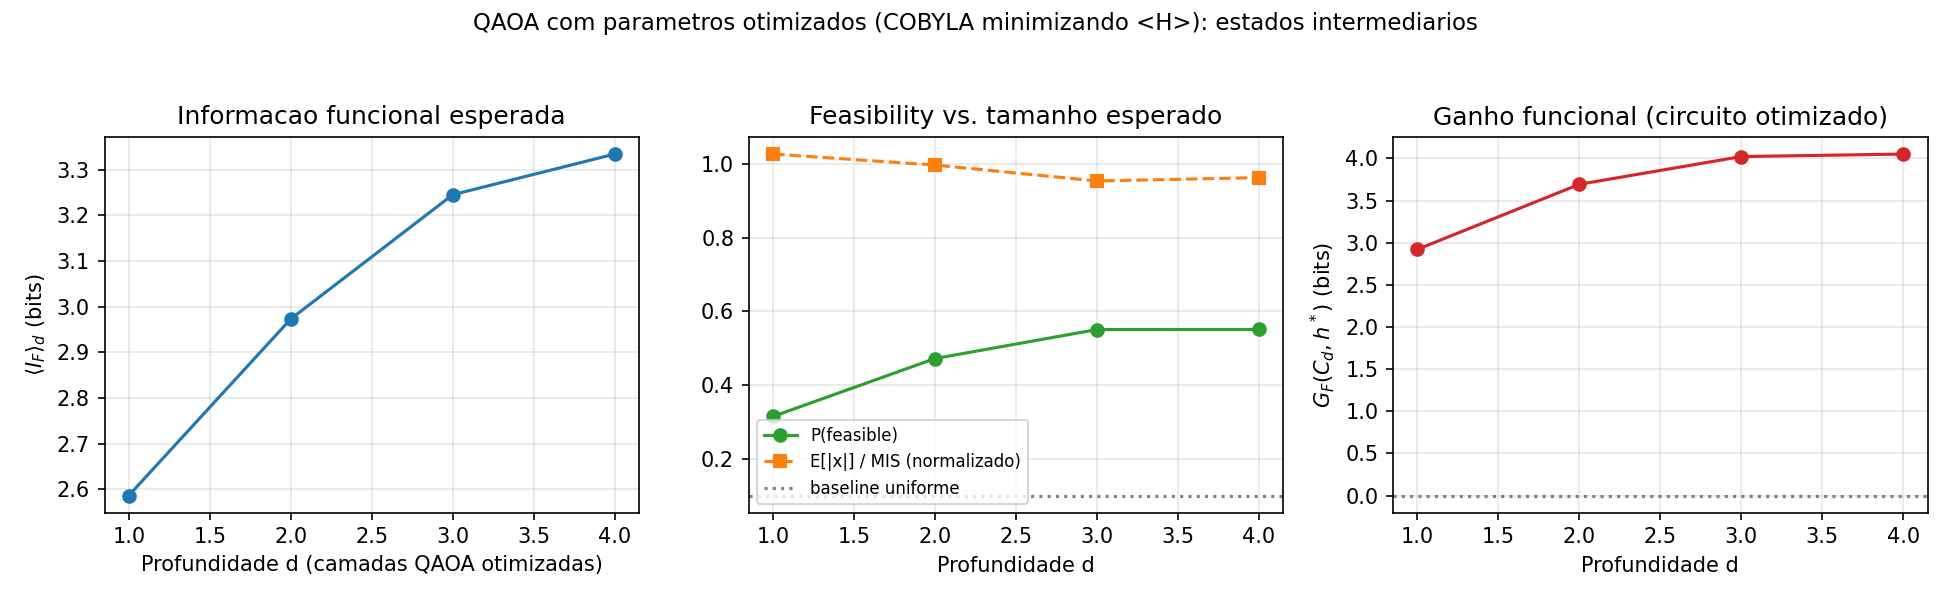
\includegraphics[width=0.85\textwidth]
    {qfi_mis_optimized_depth.png}
    \caption{
    Informação funcional esperada, viabilidade,
    tamanho esperado e ganho funcional ao longo da profundidade.
    }
    \end{figure}
}{}

\IfFileExists{qfi_mis_histogram.png}{
    \begin{figure}[H]
    \centering
    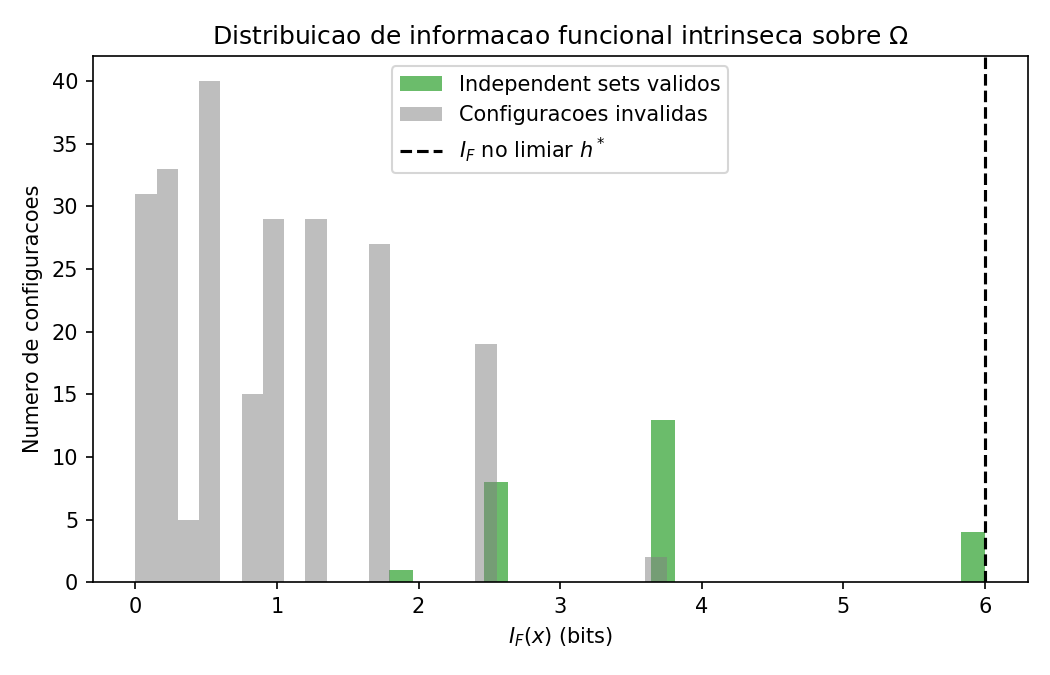
\includegraphics[width=0.85\textwidth]
    {qfi_mis_histogram.png}
    \caption{
    Distribuição de $I_F(x)$ sobre o espaço de soluções,
    separada por viabilidade.
    }
    \end{figure}
}{}

% =========================================================
\section{Perguntas de pesquisa}
% =========================================================

\begin{enumerate}[leftmargin=1.6em]

    \item Onde a informação funcional deve ser definida:
    no espaço dos circuitos ou no espaço do problema?

    \item Qual distribuição de probabilidade deve ser usada
    na fórmula de informação funcional?

    \item O que permanece fixo e o que muda durante
    a evolução do circuito?

    \item É possível atribuir informação funcional
    a cada solução candidata?

    \item A informação funcional esperada pode caracterizar
    estados intermediários?

    \item Viabilidade emerge antes de otimalidade?

    \item O circuito pode ser interpretado como amplificador
    de regiões de alta informação funcional?

    \item $\langle I_F\rangle$ revela informações que
    $\langle H\rangle$ sozinho não revela?

    \item A métrica pode ser validada sistematicamente
    em instâncias pequenas de MIS?

\end{enumerate}

% =========================================================
\section*{Proveniência das equações}
% =========================================================

\begin{definitionbox}[Literatura estabelecida]

Hazen et al.:

\[
\boxed{
I(E_x)
=
-\log_2
\left[
\frac{
M(E_x)
}{
N
}
\right]
}
\]

\end{definitionbox}

\begin{definitionbox}[Adaptação direta para MIS]

\[
\boxed{
I_F(x)
=
-\log_2
\left[
\frac{
|\{y:H(y)\leq H(x)\}|
}{
2^n
}
\right]
}
\]

Aplicação estrutural da informação funcional clássica
ao espaço de soluções do MIS.

\end{definitionbox}

\begin{proposedbox}[Métricas propostas nesta reformulação]

\[
A_F(C,h)
\]

\[
G_F(C,h)
\]

\[
\boxed{
\langle I_F\rangle_d
=
\sum_x p_d(x)I_F(x)
}
\]

\[
\Delta I_d
=
\langle I_F\rangle_d-\langle I_F\rangle_0
\]

\[
\delta I_d
=
\langle I_F\rangle_d-\langle I_F\rangle_{d-1}
\]

\end{proposedbox}

% =========================================================
\section*{Síntese}
% =========================================================

\begin{mainidea}

\centering

\textbf{\large Problema}

define

\[
I_F(x)
\]

\textbf{\large Circuito}

define

\[
p_d(x)
\]

\textbf{\large Estados intermediários}

são caracterizados por

\[
\boxed{
\langle I_F\rangle_d
=
\sum_x p_d(x)I_F(x)
}
\]

\vspace{0.3cm}

\textbf{
A paisagem funcional permanece fixa.\\
A distribuição do circuito evolui sobre ela.
}

\end{mainidea}

% =========================================================
\section*{Referências}
% =========================================================

\begin{itemize}[leftmargin=1.5em]

    \item
    Hazen, R. M., Griffin, P. L., Carothers, J. M.,
    \& Szostak, J. W. (2007).
    \emph{Functional information and the emergence of biocomplexity}.
    PNAS, 104(suppl. 1), 8574--8581.

    \item
    Wong, M. L. et al. (2023).
    \emph{On the roles of function and selection in evolving systems}.
    PNAS, 120(43), e2310223120.

    \item
    Bohm, C., Ragusa, V. R., Hintze, A., Ofria, C.,
    Dolson, E., \& Adami, C. (2026).
    \emph{Functional Information Decomposition:
    A First-Principles Approach to Analyzing Functional Relationships}.
    arXiv:2509.18522v3.

    \item
    Pasti, R., \& Krause, J. (2025).
    \emph{Quantum Functional Information through the Evolution
    of Random Circuits}.
    arXiv:2509.11409.

    \item
    Szostak, J. W. (2003).
    \emph{Functional information: Molecular messages}.
    Nature, 423, 689.

\end{itemize}

\end{document}